\chapter{Experiments}

In this chapter we demonstrate performance and comparable results of the proposed Object SLAM system with state of the art online and offline reconstruction systems in terms of trajectory accuracy and object reconstruction quality. We evaluate on the RGBD scenes V2 dataset~\cite{laiUnsupervisedFeatureLearning2014} and the TUM RGBD dataset~\cite{sturmBenchmarkEvaluationRGBD2012}, both of which are established RGBD SLAM benchmarks and compare against baseline methods.

\section{Architecture and Experimental Setup}


To support relatively high frame rate operation in the presence of slow/non-realtime deep learning components our pipeline is highly parallelized. Our system adopts the \textit{Actor} framework, where each component runs asynchronously, and communicates via thread-safe queues.

We implement the semantic segmentation pipeline as a separate python process which serializes the outputs using \texttt{protobuf} and communicates with the client thread via \texttt{zeromq} sockets in the Object SLAM pipeline. Since, instance segmentation is carried out only for keyframes, the asynchronous python process exits early (typically) freeing GPU memory, that can be used for large reconstructions.

I implement the GPU code in CUDA, and leverage the Open3D GPU framework~\cite{dongGPUAcceleratedRobust2019}. In particular, we build on the (in-house) spatially hashed TSDF implementation, implement an additional frame-to-model tracking module, and also build a back-end module for pose graph optimization. We use the optimized spherical ray-casting method to improve performance.

Our experiments were run on a Linux system (Ubuntu 18.04) with Intel i7-6700 CPU at 4.00 GHz and 32GB of RAM and a NVIDIA GTX1080 with 8GB of GPU memory.

\subsection{Qualitative results}

We first demonstrate qualitative reconstruction results on the RGBD scenes V2 dataset.  Fig.~\ref{fig:rgbd_scene13} shows the object mesh extracted from our scalable volumes with a foreground count threshold. We can see that small objects are clearly reconstructed with details, and the background is correctly filtered.

At a larger scale, Fig.~\ref{fig:objectsandscene} segments teddy bear and computers from the cluttered scene and ensures a low-drift of the trajectory. Fig.~\ref{fig:rgbd_scene12} compares reconstructions from \textit{MaskFusion} \cite{runz_maskfusion_2018} and our system for a given sequence. It can be seen that the object-level reconstruction, specifically for caps and sofas, is much cleaner by our system than by \textit{MaskFusion}.

%that our system can mostly prune background wall and floors, while keeping the segmented sofa and table in the scene reconstruction.

\subsection{Quantitative results}

Table \ref{tab:ATE_RMSE} presents Absolute Trajectory Error (ATE) of four different methods compared with our system. Note in the table, the best results of \textit{the object-based systems} are in \textit{bold}, and provide results from geometric SLAM systems for reference.

In general, we achieve comparable results against the state-of-the-art surfel based online SLAM system \textit{ElasticFusion}~\cite{whelan2016elasticfusion} and volumetric offline reconstruction system \textit{Open3D}~\cite{zhou_open3d_2018}. In the meantime, our method outperforms object-based SLAM systems \textit{MaskFusion}\footnote{MaskFusion requires 2 high end graphics cards to run it in online mode. We ran it in offline mode, and stored all the detected object instances from the method instead of manually selecting objects of interest for a fair comparison with our method}~\cite{runz_maskfusion_2018}
and \textit{Fusion++} \footnote{Fusion++ is not open sourced and we obtained the results from the paper.}\cite{fusionPP} by a large margin. This improvement can be attributed to the use of semantic data association and scalable voxel grids.

For small scenes in the \textit{RGB-D scenes V2 dataset}, we achieve consistently high accuracy with ATE below $5cm$ for all scenes. Figure~\ref{fig:rgbd_scenes-ape} shows detailed trajectory visualizations.

For larger scenes, although noisy semantic segmentations affect masks and introduce noise for frame-to-model odometry, compositional rendering still ensures reliable tracking. Trajectory comparisons are provided in Figure~\ref{fig:fr3_household-ape}.


\begin{figure}[t!]
    \centering
    \subfloat[\label{sfig:obj_loop_closure_a}]{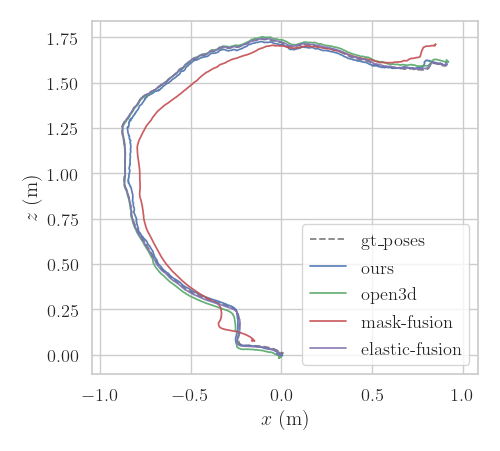
\includegraphics[width=0.8\linewidth]{figs/scene12-ape.png}}\\
    \subfloat[\label{sfig:obj_loop_closure_b}]{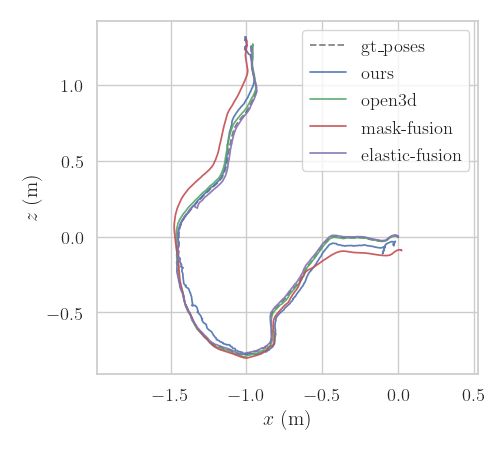
\includegraphics[width=0.8\linewidth]{figs/scene14-ape.png}}
    \caption{Comparison of trajectories between our pipeline and baselines with ground truth. (a) shows \emph{rgbd-scenes-v12} and (b) shows \emph{rgbd-scenes-v14} sequences. }
    \vspace*{-1em}
    \label{fig:rgbd_scenes-ape}
\end{figure}
